{$\space$\par}
\vspace{0.5cm}
\justifying
\section*{{\bfseries \LARGE Questão 2 -} {\bfseries \large Com base nessas notas, você diria que o CRA do primeiro período é uma função linearmente proporcional ao desempenho do aluno no ENEM?}}

\vspace{0.2cm}

\textcolor{red}{Para analisar rigorosamente, irei fazer um ajuste linear simples e obter o valor p. A minha métrica de desempenho para o ENEM será apenas a média ponderada, onde assumirei peso igual para todas matérias.}


\begin{lstlisting}
    install.packages('MASS')
    library(MASS)
    
    # Data
    enem_mean = rowMeans(astro[,c(2:6)])
    cra = astro$CRA
    
    # Reg
    reg = lm(cra ~ enem_mean,method='MM')
    summary(reg)
    
    ### output ### 
    Call:
    lm(formula = cra ~ enem_mean, method = "MM")
    
    Residuals:
        Min      1Q  Median      3Q     Max 
    -3.0514 -0.9285  0.1149  1.2654  1.8299 
    
    Coefficients:
                 Estimate Std. Error t value Pr(>|t|)  
    (Intercept) -7.965886   5.982551  -1.332   0.2017  
    enem_mean    0.021012   0.008508   2.470   0.0252 *
    ---
    Signif. codes:  0 ‘***’ 0.001 ‘**’ 0.01 ‘*’ 0.05 ‘.’ 0.1 ‘ ’ 1
    
    Residual standard error: 1.525 on 16 degrees of freedom
    Multiple R-squared:  0.276,	Adjusted R-squared:  0.2308 
    F-statistic:   6.1 on 1 and 16 DF,  p-value: 0.02515
    
    # Plot
    x = c(min(enem_mean):max(enem_mean),100)
    plot(enem_mean, cra, cex=2.5, col='red',pch=16,xlab='Média ENEM',
         ylab='CRA',cex.lab=2.5,cex.axis=2) 
    abline(reg, col='blue', lwd=3)
    legend('topleft',legend=c('Alunos','Ajuste linear'),col=c('red','blue'),
    pch=c(16,NA),lty = c(NA, 1),lwd = c(NA, 3),cex=c(1.5,1.5),bty='n')
    
    # Text
    text(640, 3.5, paste('Correlacao (Spearman):', correlation, "\n p-valor:",
     round(test$p.value,3)),
         cex=2.5,
         font=2)
\end{lstlisting}

\begin{figure}
    \centering
    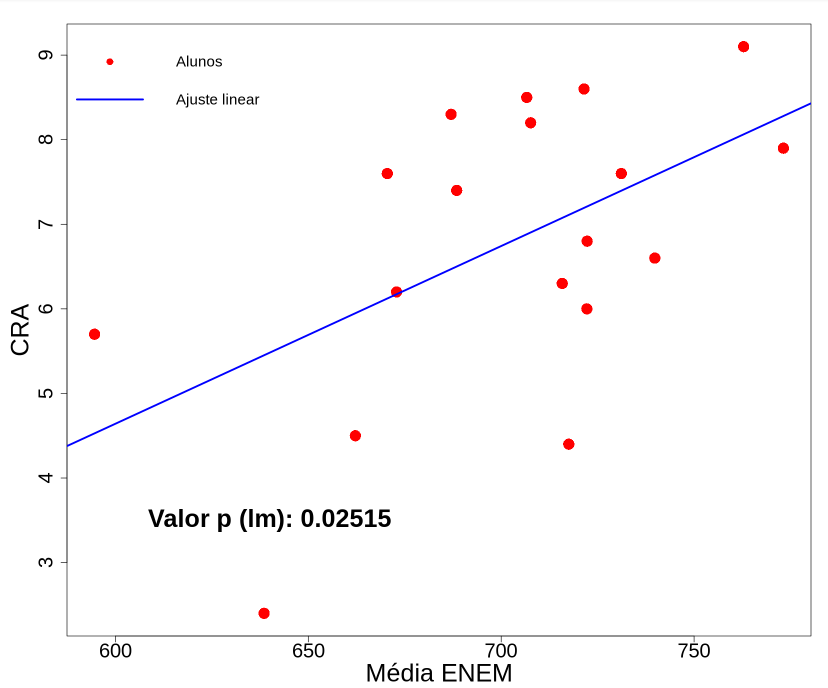
\includegraphics[width=0.8\linewidth]{Figuras/corr_enem.png}
    \caption{CRA em função da média ponderada no ENEM dos alunos da astronomia das turmas de 2024 e 2025.}
    \label{corr_enem}
\end{figure}


\textcolor{red}{Ao observar o valor p do modelo linear na figura \ref{corr_enem}, não podemos fazer nenhuma afirmação sobre a linearidade entre o CRA e o desempenho no ENEM.}